\section{\eTrice{} Models and Their Relations}

\eTrice{} comprises several models:

\begin{itemize}
\item the ROOM model (*.room) -- defines model classes and the logical structure of the model
\item the Config model (*.config) -- defines configuration values for attributes
\item the Physical model (*.etphys) -- defines the structure and properties of the physical system
\item the Mapping model (*.etmap) -- defines a mapping from logical elements to physical elements
\end{itemize}

In the following diagram the models and their relations are depicted. The meaning of the arrows is: 
uses/references.

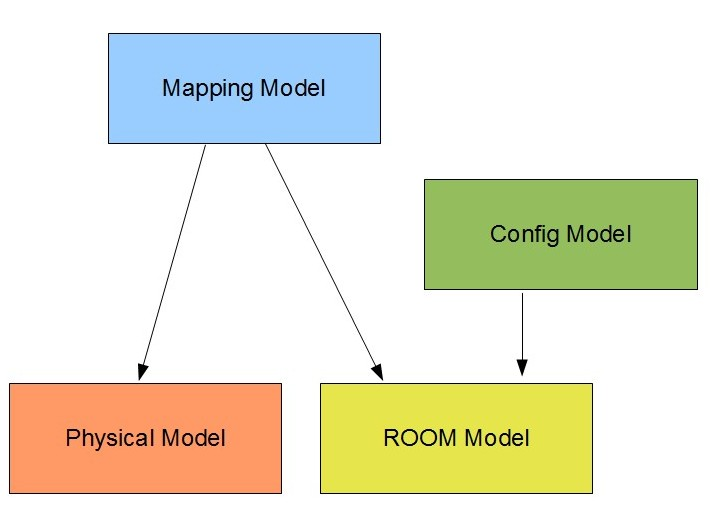
\includegraphics[scale=0.4]{images/080-models.jpg}

In the following sections we will describe those models with emphasis of their cross relations.

\subsection{The ROOM Model}

The ROOM model defines \room{DataClass}es, \room{ProtocolClass}es, \room{ActorClass}es, \room{SubSystemClass}es and \room{LogicalSystem}s.
Thereby the three latter form a hierarchy. The \room{LogicalSystem} is the top level element of the structure. 
It contains references to \room{SubSystemClass} elements. The \room{SubSystemClass} in turn contains 
references to \room{ActorClass} elements which again contain (recursively) references to 
\room{ActorClass} elements. The complete structural hierarchy implies a tree which has the 
\room{LogicalSystem} as root and where each reference stands for a new node with possibly further 
branches.

Let's consider a simple example. It doesn't implement anything meaningful and completely omits behavioral and 
other aspects.

\lstinputlisting[language=ROOM, caption={ROOM example code}, label={lst:room_example}]{../model/room-example.room}

When a \room{LogicalSystem} is instantiated then recursively all of the contained referenced elements are 
instantiated as instances of the corresponding class. Thus the instance tree of the above example looks like 
in figure \ref{fig:instance_tree} (the third line in the white boxes shows some mapping information,
see section \ref{sec:mapping_model} \nameref{sec:mapping_model}):

\begin{figure}
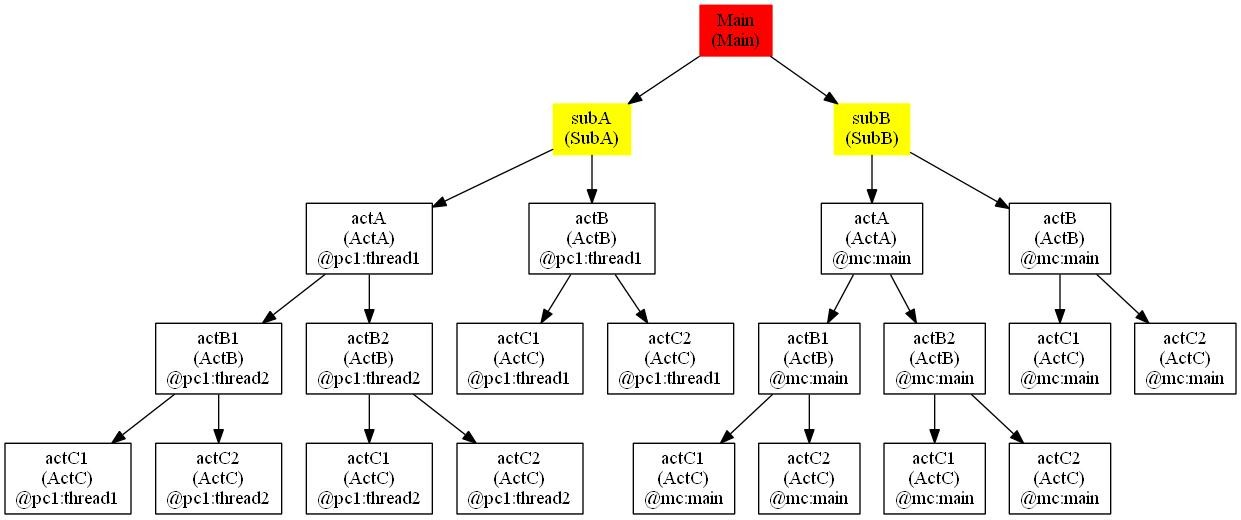
\includegraphics[scale=0.45]{images/080-instances.jpg}
\caption{Instances of a ROOM system}
\label{fig:instance_tree}
\end{figure}

\subsection{The Config Model}

Once we have the ROOM class model we can configure values using the Config model. This can be done on the 
class level and/or on the instance level. Values defined for class attributes are used for all instances 
unless there is an instance value configured for the same attribute.

\lstinputlisting[language=Config, caption=Config example code]{../model/config-example.config}

\subsection{The Physical Model}

The physical model defines the physical resources onto which the logical system will be deployed. It is 
possible to define runtime classes which (currently) only define the overall execution model of the 
platform.

\lstinputlisting[language=etPhys, caption=etPhys runtime definition]{../model/etphys-runtimes.etphys}

The \room{PhysicalSystem} is composed of \room{NodeRef}erences which are instances
of \room{NodeClass}es. Each \room{NodeClass} is referencing a 
\room{RuntimeClass} and is defining \room{Threads}.

\lstinputlisting[language=etPhys, caption=etPhys example code]{../model/etphys-example.etphys}

\subsection{The Mapping Model}
\label{sec:mapping_model}

The last model finally combines all this information by mapping logical to physical entities.

\lstinputlisting[language=etMap, caption=etMap example code]{../model/etmap-example.etmap}

The result of the mapping is also depicted in above tree diagram (figure \ref{fig:instance_tree})
of the instances. All actor instances (the white boxes) are mapped to a node and a thread running on this node
(shown as @\textit{node} : \textit{thread}).

